\documentclass[12pt]{article}

\usepackage[utf8]{inputenc}
\usepackage[T1]{fontenc}
\usepackage{lmodern}
\usepackage{amsmath}
\usepackage{mathtools}
\usepackage{amssymb}

\usepackage{syntax}
\setlength{\grammarindent}{3em}

\usepackage{natbib}
% \usepackage{xcolor}
\usepackage[hidelinks]{hyperref}
\usepackage{algorithm}
\usepackage[noend]{algpseudocode}
% \usepackage{algorithmicx}
\usepackage{graphicx}
\usepackage{animate}
\usepackage{booktabs}
\usepackage{tabulary}
\usepackage{rotating}
\usepackage{pgfgantt}

% Algorithm stuff
\makeatletter
\newcounter{algorithmbis}
\setcounter{algorithmbis}{0}
\renewcommand{\thealgorithmbis}{\arabic{algorithmbis}}
\def\algorithmbis{\@ifnextchar[{\@algorithmbisa}{\@algorithmbisb}}
\def\@algorithmbisa[#1]{%
  \refstepcounter{algorithmbis}
  \trivlist
  \leftmargin\z@
  \itemindent\z@
  \labelsep\z@
  \item[\parbox{\textwidth}{%
    \hrule
    \hrule
    \noindent\strut\textbf{Algorithm \thealgorithmbis} #1
    \hrule
  }]\hfil\vskip0em%
}
% \newcommand*{\oldeqref}{}
% \let\oldeqref\eqref
% \renewcommand*{\eqref}[1]{%
%   \begingroup
%     \hypersetup{
%       linkcolor=linkequation,
%       linkbordercolor=linkequation,
%     }%
%     \oldeqref{#1}%
%   \endgroup
% }
\def\@algorithmbisb{\@algorithmbisa[]}
\def\endalgorithmbis{\hfil\vskip-1em\hrule\endtrivlist}
\makeatother

% Math stuff
\DeclareMathOperator*{\argmin}{arg\,min}
\DeclareMathOperator*{\argmax}{arg\,max}
\DeclareMathOperator{\Bin}{Bin}
\DeclareMathOperator{\Ber}{Ber}
\DeclareMathOperator{\Beta}{Beta}
\DeclareMathOperator{\BetaBin}{BetaBin}
\DeclareMathOperator{\Cat}{Cat}
\DeclareMathOperator{\Dir}{Dir}
\DeclareMathOperator{\DirMult}{DirMult}
\DeclareMathOperator{\Mult}{Mult}
\DeclareMathOperator{\Poi}{Poi}
\DeclareMathOperator{\Gammadist}{Gamma}
\DeclareMathOperator{\NB}{NB}
\DeclareMathOperator{\Unif}{Unif}
\DeclareMathOperator{\Pareto}{Pareto}
\DeclareMathOperator{\Gauss}{\mathcal N}
\DeclareMathOperator{\E}{\mathbb{E}}
\DeclareMathOperator{\var}{\mathrm{var}}
\DeclareMathOperator{\cov}{\mathrm{cov}}
\DeclareMathOperator{\grad}{\mathrm{grad}}
\newcommand*\mean[1]{\bar{#1}}
\DeclareMathOperator{\diag}{diag}
\newcommand{\KL}[2]{D_{\text{KL}}\left(#1 \Vert #2\right)}
\DeclareMathOperator{\Tr}{Tr}
\DeclareMathOperator{\DP}{DP}
\DeclareMathOperator{\GP}{GP}
\DeclareMathOperator{\GEM}{GEM}
\DeclareMathOperator{\I}{\mathbb I}
\DeclareMathOperator{\pa}{pa}
\let\oldemptyset\emptyset
\let\emptyset\varnothing
\newcommand{\at}[2][]{#1|_{#2}}
\newcommand{\given}{\mid}

% bold vectors
\renewcommand{\vec}[1]{\boldsymbol{\mathbf{#1}}}

% Theorem, proofs, etc.
\usepackage{amsthm}
\usepackage{thmtools}
\makeatletter
\def\thm@space@setup{%
  \thm@preskip=\parskip \thm@postskip=0pt
}
\makeatother
\theoremstyle{definition}
% \newtheorem{definition}{Definition}[section]
\declaretheorem[qed=$\triangle$,numberwithin=section]{definition}
\newtheorem{theorem}{Theorem}[section]
\newtheorem{proposition}{Proposition}[section]
\newtheorem{claim}{Claim}[section]
% End with a triangle
\declaretheorem[qed=$\triangle$,sibling=definition]{example}

% Double spacing
\usepackage{setspace}
\doublespacing

% Margins
\usepackage[margin=2cm,a4paper]{geometry}

% Change font to Times New Roman
\usepackage{mathptmx}

% No indent, but skip paragraphs
\usepackage[parfill]{parskip}

% 1st, 2nd, 3rd, 4th, etc.
\usepackage[super]{nth}

% including code
\usepackage{listings}
\lstset{
  captionpos = b,
  numbers = left,
  frame = single,
  basicstyle = \ttfamily,
  lineskip = -3pt
}

% no itemsep
\usepackage{enumitem}
\setlist{noitemsep, topsep=-5pt}

% verbatim font size
% \makeatletter
%   \def\verbatim{\huge\@verbatim \frenchspacing\@vobeyspaces \@xverbatim}
% \makeatother

\usepackage{cleveref}
\newcommand\creflastconjunction{, and\nobreakspace} % Oxford comma
\crefname{appendix}{Appendix}{Appendices}
\crefname{section}{Section}{Sections}
\crefname{figure}{Figure}{Figures}
\crefname{table}{Table}{Tables}

% subfig
\usepackage{subcaption}

% for including pdfs
\usepackage{pdfpages}

% for titlepage
\newcommand{\HRule}{\rule{\linewidth}{0.5mm}}

\title{\vspace{-50pt} Scaling Probabilistic Programming to Structured Spaces}
\author{}
\date{}

\begin{document}

\begin{titlepage}
\begin{center}

% Upper part of the page. The '~' is needed because \\
% only works if a paragraph has started.
~\\[2cm]

\textsc{\LARGE Transfer of Status Report}\\[2cm]


\includegraphics[width=0.3\textwidth]{oxford.pdf}\\[2cm]

\textsc{\Large University of Oxford}\\
\textsc{\Large Department of Engineering Science}\\[2cm]


% Author and supervisor
\begin{minipage}{0.4\textwidth}
\begin{flushleft} \large
\emph{Author:}\\
Robert Zinkov\\
\end{flushleft}
\end{minipage}
\begin{minipage}{0.4\textwidth}
\begin{flushright} \large
\emph{Supervisor:} \\
Frank \textsc{Wood}
\end{flushright}
\end{minipage}

\vfill

% Bottom of the page
{\large Michaelmas 2018}

\end{center}
\end{titlepage}

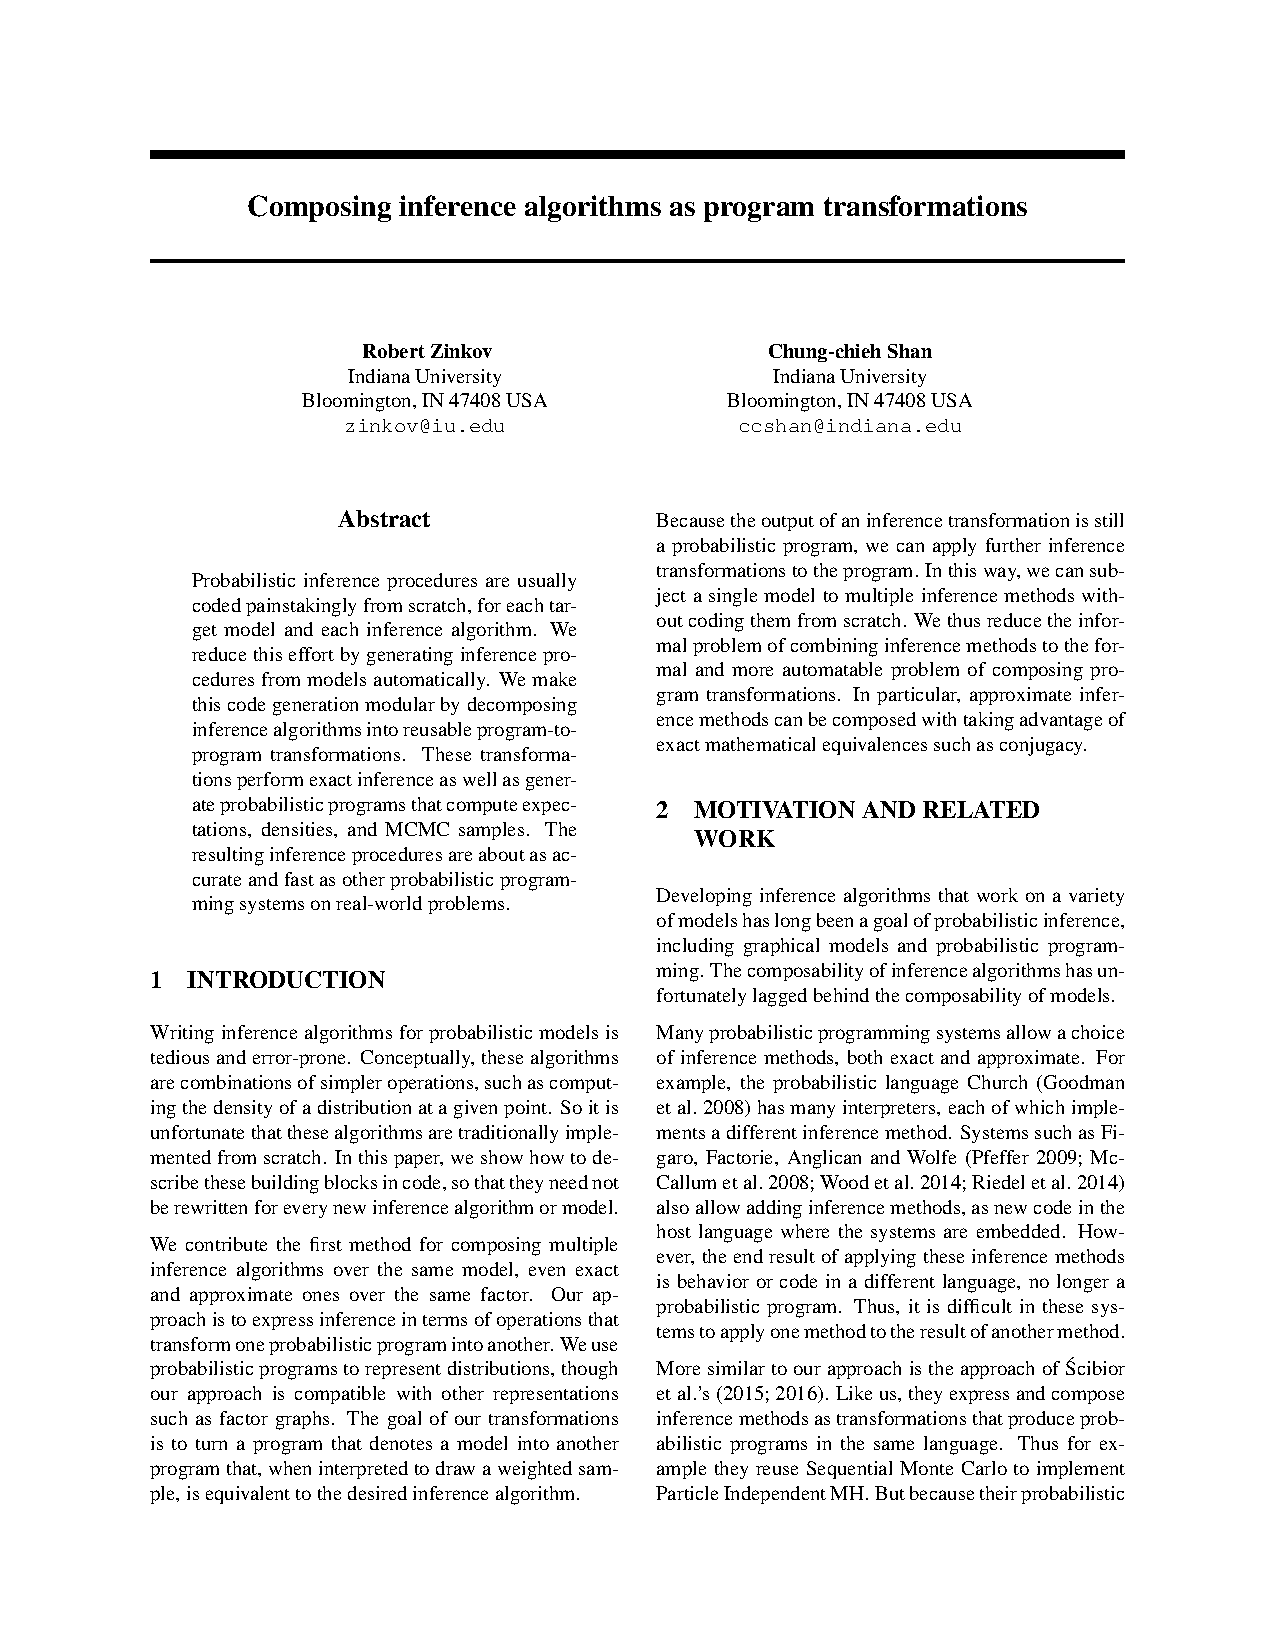
\includepdf[pages=-]{multi.pdf}

\vspace{-2em}
\maketitle
\vspace{-5em}	
	
\doublespacing	
	
\setlength{\belowdisplayskip}{12pt} \setlength{\belowdisplayshortskip}{12pt}
\setlength{\abovedisplayskip}{12pt} \setlength{\abovedisplayshortskip}{12pt}


\section{Introduction}

In this report, we introduce and review the necessary background
material around probabilistic programming, the existing literature for
performing inference in the models expressible with probabilistic
programming languages, and propose mechanisms extending existing
probabilistic programming systems so that models are easier to debug
and may then be applied to more challenging probabilistic modelling
tasks.

\section{Literature Review}

\subsection{Probabilistic Programming}

Probabilistic programming systems \citep{gordon2014probabilistic}
are specialised systems for specifying probabilistic models and
efficiently performing inference with them. These models are usually
expressed in a domain specific language (DSL) called a probabilistic
programming language (PPL). These restricted languages are more
amendable to program analysis and offer the potential of more easily
generating efficient inference code for a particular model.




\subsubsection{Taxonomy of Probabilistic Programming systems}

Probabilistic programming languages can be partitioned into two
designations: \emph{first-order} PPLs and \emph{higher-order} PPLs.
First-order PPLs are ones where we can statically determine the number
of latent variables of the model without performing any inference. The
most popular systems are first-order as these restrictions make it
possible to apply efficient inference algorithms to all models
expressible within them. First-order PPLs include BUGS
\citep{lunn2000winbugs}, Infer.NET \citep{InferNET14}, Stan
\citep{carpenter2015stan}, PyMC \citep{salvatier2016probabilistic}, as
well as Edward \citep{tran2016edward}.

Higher-order PPLs are languages which can express all the
probabilistic models that first-order PPLs are unable to. This greater
flexibility in specification comes with a greater challenge in
devising generic inference algorithms that can be made to work in this
larger model family. In the literature higher-order PPLs are sometimes
referred to as universal probabilistic programming languages
\citep{infcomp2017, yang2014generating} or languages with recursion.

It is deceptive to state that the defining characteristic of
higher-order PPLs is that the languages have recursion as the
recursion is only a problem if within recursion we make draws from a
distribution. A fully deterministic recursive function is perfectly
acceptable to use in a first-order PPL. This is indeed the case
in the Stan language.

When our model has an unfixed number of latent variables, this introduces
the additional challenge that we need to be able generate unique names
for them as we sample from our model. This process of generating names
is called an \emph{addressing scheme}.

The addressing scheme is important for implementing MCMC algorithms where
we need to maintain which of the latent variables in our proposed state
are shared with variables in our current state.

\subsubsection{Core language grammar}

To keep things concrete we introduce a small language \textsc{Hakaru}.
We define this grammar we more formally in \cref{fig:coregrammar}.

\begin{figure}
\begin{grammar}
  <e> ::= <x> | "1" | <e> "-" <e> | <e> "<" <e> | "exp("<e>")" | "If("<e>","<e>","<e>")" | \dots
\alt "Sum("<e>","<e>","<x>","<e>")" | "Int("<e>","<e>","<x>","<e>")"
\alt "Lam("<x>","<e>")" | "App("<e>","<e>")" | "("<e>","<e>")" | <e>"[0]" | <e>"[1]"
\alt "Uniform("<e>","<e>")" | "Normal("<e>","<e>")"
\alt "Gamma("<e>","<e>")" | "Weight("<e>","<e>")"
\alt "Categorical(("<e>","<e>"), \dots)"
\alt "Superpose(("<e>","<e>"), \dots)" | <x>"\,<~\,"<e>"\,;\,"<e>
\end{grammar}
\caption{Grammar for the core of a probabilistic programming language}
\label{fig:coregrammar}
\end{figure}

\subsubsection{Importance sampler}

The simplest inference algorithm to implement for higher-order PPLs is
an importance sampling algorithm. This algorithm is also called likelihood-weighting.

This inference algorithm is first implemented in the BLOG
probabilistic programming system \citep{milchijcai2005}.

\subsubsection{Trace MH interpreter}

Up until recently, the most common inference algorithm which came with
probabilistic programming systems is a single-site Metropolis Hastings
called Trace MH
\citep{scibior2018functional,wingate2011lightweight}. In this
algorithm, we generate run the program instrumented to keep track of
all random variables we encountered.  Then we re-execute the program in
such a way that all but one of the random variables is kept fixed. This
has the possibility of creating and removing random variables based on
changes in control-flow.

\subsubsection{SMC interpreter}

Another popular to implement inference algorithm for probabilistic
programming systems is the SMC interpreter \citep{wood2014new}. In
this setting, we generate a large population of particles and as
we execute the trace we re-weight them based on which of the random
variables we encounter are observed.

\subsubsection{Variational and Amortised Inference}

Variational inference encompasses a family of inference techniques
centred around posing inference problems as optimisation problems. The
idea being that we can construct a parameterised family of approximate
distributions $q(\vec x; \phi)$ and then finding the $\phi$ closest to
probability distribution we actually care about. The notion of closest
is often some f-divergence and mostly commonly the reverse KL divergence.

\begin{equation}
  \KL{q(\vec x; \phi)}{p(\vec x)} \coloneqq \E_{q(\vec x; \phi)} \left[ \log q(\vec x) - \log p(\vec x; \phi) \right]
\end{equation}

This KL divergence can be then be rewritten as:

\begin{equation}
  \KL{q(\vec x \given \vec y; \phi}{p(\vec x \given \vec y)} = \E_{q(\vec x \given \vec y; \phi)} \left[ \log p(\vec x, \vec y) - \log q(\vec x \given \vec y; \phi) \right]
\end{equation}

This is called the Evidence Lower Bound (ELBO).

The idea with amortised inference \citep{gershman2014amortized} is that we can share parameters $\phi$ for different choices of $\vec x$.

\subsubsection{Variational Autoencoders}

We can further generalise the amortised inference regime to allow us to
jointly learn the model from the data as well the approximation of
the posterior for the model.

\subsection{Compiled Inference}

Stochastic variational inference methods assume taking draws from an
approximate distribution is easier than taking draws from the true
distribution. But if the joint distribution of the true distribution
is easy to draw samples from, there is an formulation of the KL
divergence that we may use for amortised inference.

\begin{align}
  \begin{split}
    \mathcal{L}(\phi) & = \E_{p(\mathbf{y})}\left[\KL{p(\vec x \given \vec y)}{q(\vec x \given \vec y; \phi)})\right] \\
    & = \E_{p(\vec x, \vec y)} \left[-\log q(\vec x \given \vec y; \phi)\right] + \text{const}
  \end{split}
\end{align}

\subsection{Implicit Models}

For many of the models we can express in a probabilistic programming
system, we are unable to efficiently compute the density of a trace
associated with our model. For example, in large physics and
biological simulators it can be computationally intractable
to compute a density.

\subsection{Model criticism}

As part of defining and performing inference on our probabilistic
models, we often want to evaluate our models. If our models when
fitted can be used to make predictions, we can evaluate their accuracy
on held-out labelled data, but this is inappropriate for many
settings. More generally, if we have unlabelled data we may evaluate
the test likelihood of it under our proposed model.

\subsubsection{Two Sample Kernel Tests}

Another approach, is to suppose we have our data $Y$ and data
generated after fitting $Y^\prime$. We can ask if $Y$ and $Y^\prime$
appear to come from the same distribution.

We can pose this statistic as a maximum mean discrepancy \citep{gretton2012kernel} (MMD).

\section{Proposal}

The common thread that underlies this project is to push probabilistic
programming to be applied in new settings that can take advantage of these
new scalable inference algorithms as well as make the systems for usable
for non-experts.

\subsection{Debugging Probabilistic Programming}

Often probabilistic modeling is an iterative process where a user
tries out a model, evaluates it in some way, and then proposes some
improvement. We can aid in the process by offering suggestions automatically
for ways to improve a probabilistic model.

The main idea is to define a neighbourhood $\mathcal{N}(p)$ which are
the set of programs we can get to from our current program $p$ by a
set of known pre-defined rewrites.

An example of some possible rewrites could be:
\begin{itemize}
\item Replace $e_1 \sim \text{Normal}(e_2, e_3)$ with $e_1 \sim \text{Laplace}(e_2, e_3)$
\item Replace $e_1 \sim e_2$ with $e_1 \sim \text{Mix}(e_2, \delta(0))$ where Mix is a mixture distribution  
\end{itemize}

Each of these proposed programs can then be fitted and compared with
the original program using a two-sample kernel test. We can then present
the choices to the user interactively through some UI element in the PPS.

This work is most similar to work by \citet{grosse2012a}. The two main
differences between this work and theirs is they restrict their search
to a smaller space around a context-free grammar designed to mimic how
humans heuristically choose to augment their probabilistic model,
which means it can not discover. Additionally, their goal is to
greedily discover the best structure while, we are more interesting in
this as a debugging and diagnostic tool. In that sense, we are not
doing a greedy search through the space of probabilistic programs as
much as a quick exploration of the local neighbourhood of programs
around the one the user has provided.

We mitigate the risks of this project by first restricting ourselves
to a small subset of possible changes to the probabilistic model. This
makes it more likely that we will find changes which improve the model
while spending less computational time exploring the space of
programs.  I will further collaborate with my other supervisor Dino
Sejinovic, who is an expert in using kernel methods like MMD for
hypothesis testing.

\subsection{Data Cleaning}

While most research focuses on the model fitting and evaluation steps
in data analysis, most of the time of practitioners is spent on
acquiring and cleaning the datasets. Data cleaning can describe
writing transformations to get data into a proper schema, correcting
annotation errors, removing duplicates, as well correcting other
internal inconsistencies. This project focuses on data which is
already in a tabular format, is likely to mostly fit into a schema
unknown in advance, but may still have errors and misspellings that
need to be corrected.

The approach we take is defining a generative model for tabular data
where we define a prior on data schema, and a generative model for
generating cells of data conditioned on this schema as well as
previously generated cells.

We mitigate the risks of this project by initially restricting
ourselves to synthetically-generated tabular datasets as well previous
real-world noisy tabular data where a prior analysis has given us some
ground truth to work with.


\subsection{Automated Expectation Maximisation}

Probabilistic programming systems can also be extended to do more than
sample from a conditional distribution.

We mitigate the risk of this project in starting with a restricted
model family of conditionally conjugate models where we know the
exact rewrites our computer algebra system will need to do.

\subsection{Proposed Schedule of Work}

The timeline we are proposing for this study consists of submitting
the preliminary work on debugging probabilistic programs and Bayesian
metalearning to an appropriate NIPS workshop. If we are exceedingly
lucky in obtaining results we will submit this work to AISTATS on
October 4th. Otherwise, it is more likely that this work will be
submitted to UAI in March. The data cleaning project is intended to be
submitted to the KDD conference.

\begin{figure}[h]
	\centering
	\begin{ganttchart}[
		y unit title=0.65cm,
		y unit chart=0.65cm,
		x unit = .35cm,
		vgrid,
		hgrid,
		inline,
		%link/.style={->, line width=0.7pt, red},
		% time slot format=isodate,
		% today=2,
		% today offset=0.5,
		% today label=Start of Michaelmas,
		% today label node/.append style={anchor=north west},
		% today label font=\itshape,
		% today label font=\small,
		% today rule/.style={draw=blue, ultra thick},
		%
		bar label font=\scriptsize,
		%
		title label node/.style={anchor=mid,font=\small}, %,below=-1.6ex},
		%title left shift=.0,
		%title right shift=0.0,
		%title top shift=0.1,
		title height=1,
		%title label font=\small,
		%bar/.style={fill=gray!50},
		%incomplete/.style={fill=white},
		bar/.append style={fill=gray!50,draw=none},
		bar incomplete/.append style={fill=gray!25,draw=none},
		progress label text={},
		bar height=0.8,
		bar top shift=0.1,
		% group right shift=0,
		% group top shift=.6,
		% group height=.3,
		milestone/.append style={fill=cyan, shape=ganttmilestone},
		%milestone label font =\scriptsize,
		milestone inline label node/.style={anchor=east,font=\footnotesize},
		milestone height = 0.3,
		milestone top shift = 0.35,
		milestone left shift = 0.65,
		milestone right shift = 0.35,
		%group right shift=0,
		%group top shift=0.6,
		%group height=0.3,
		%group peaks height =0.2
		]{1}{48}
		%labels
		\gantttitle{2018--2019}{48} \\
		\gantttitle{Sep.}{4} 
		\gantttitle{Oct.}{4} 
		\gantttitle{Nov.}{4} 
		\gantttitle{Dec.}{4} 
		\gantttitle{Jan.}{4} 
		\gantttitle{Feb.}{4}
		\gantttitle{Mar.}{4}
		\gantttitle{Apr.}{4}
		\gantttitle{May}{4} 
		\gantttitle{Jun.}{4}
		\gantttitle{Jul.}{4}
		\gantttitle{Aug.}{4} \\
		%tasks
		\ganttmilestone{AISTATS }{5}
		\ganttmilestone{NIPS W.}{10}
		\ganttmilestone{ICML }{18}
                \ganttmilestone{KDD }{23}
		\ganttmilestone{UAI }{27}
		\ganttmilestone{NIPS }{36}
		\\ %ICML
		\ganttbar[progress=20]{Debugging probabilistic programs}{1}{10} \\
		\ganttbar[progress=10]{Data Cleaning}{1}{23} \\
                \ganttbar[progress=5]{Bayesian Meta-learning}{3}{27} \\
                %\ganttbar[progress=0]{Program synthesis}{18}{36} \\
		\ganttbar[progress=0]{New research directions}{27}{48}
		%% \ganttlink{elem5}{elem7}
		%% \ganttlink{elem6}{elem7}
	\end{ganttchart}
	\vspace{-0.4cm}
	\caption{Proposed plan for the upcoming year. Conference deadlines are marked on the first row}
	\label{fig:gantt}
\end{figure}

\pagebreak
	
\bibliographystyle{unsrtnat}
{\small \singlespacing
	\bibliography{report}}


\end{document}

%%  LocalWords:  Sejinovic
